\section{Results and Discussion}
\label{sec:results}

All results are on the ETTh1 test split (2,785 windows, horizon 96, scaled units) and are means over two seeds unless stated otherwise. Table~\ref{tab:headline} gives the headline comparison between the baseline and the full model with the per-seed values; Tables~\ref{tab:groups-mse} to~\ref{tab:delta-a1} break the results down by corruption family and variant, and Appendix~\ref{app:full} lists every condition.

\begin{table}[!t]
\centering
\caption{Headline Results: PatchTST (A0) Versus RA-PatchTST (A4)}
\label{tab:headline}
\footnotesize
\colfit{%
\begin{tabular}{@{}llccl@{}}
\toprule
Model & Test condition & MSE & MAE & Per-seed MSE \\
\midrule
\tabin{tab_headline}
\bottomrule
\end{tabular}}
\end{table}

\subsection{Clean-Data Reproduction (O1)}

Table~\ref{tab:repro} reports the clean test error of each variant with the checkpoint chosen on clean validation loss, which is how PatchTST is usually evaluated. The baseline A0 reaches MSE 0.3791 and MAE 0.4008, against 0.375 and 0.399 published for PatchTST/42~\cite{patchtst}, a gap of 1.1\% in MSE and 0.5\% in MAE, which meets the 2\% target. The remaining gap is plausibly due to the shorter training budget: seed 2021 of A0 reached its best validation score in the last allowed epoch (Table~\ref{tab:cost}), so it had not finished improving. In every run the two checkpoint rules happened to select the same epoch, so the clean numbers in Tables~\ref{tab:headline} and~\ref{tab:repro} coincide.

\begin{table}[!t]
\centering
\caption{Clean Test Error With the Clean-Validation Checkpoint, Against the Published PatchTST/42 Result (MSE 0.375, MAE 0.399)}
\label{tab:repro}
\footnotesize
\colfit{%
\begin{tabular}{@{}lcccc@{}}
\toprule
Variant & MSE & MAE & $\Delta$MSE vs.\ paper & $\Delta$MAE vs.\ paper \\
\midrule
\tabin{tab_repro}
\bottomrule
\end{tabular}}
\end{table}

\subsection{How Much Does Corruption Hurt PatchTST? (RQ1)}

The baseline degrades very unevenly across corruption families (first column of Table~\ref{tab:groups-mse}, Fig.~\ref{fig:groups}). Point-wise missing values, 16-step stretches and noise raise its MSE by only 0.005 to 0.013 on average, and even at 15\% the worst of them costs 7\% (missing stretches, 0.406). Spikes raise the mean MSE to 0.458 ($+20.9\%$) and segment-level shift to 0.520 ($+37.1\%$); at ten shifted segments the MSE reaches 0.712, 88\% above the clean value. Averaged over all 21 corrupted conditions the baseline loses 13.3\%.

Instance normalization explains most of this pattern. A zero in a scaled series is the training mean, which instance normalization turns into a moderate value, and Gaussian noise of one standard deviation on a few percent of the points barely changes the window statistics. A spike of 3 to 5 standard deviations, on the other hand, inflates $\sigma_c$ in~\eqref{eq:revin}, which compresses every other value of the window after normalization and then stretches the forecast when the statistics are restored. A shifted segment moves both $\mu_c$ and $\sigma_c$ and changes the local shape that the patches encode. In both cases the damage spreads, through the window statistics, to every patch of the window.

\begin{table*}[!t]
\centering
\caption{Test MSE by Corruption Family (Mean $\pm$ Standard Deviation Over Two Seeds; Best in Bold)}
\label{tab:groups-mse}
\footnotesize
\begin{tabular}{@{}lccccc@{}}
\toprule
Test condition & A0 PatchTST & A1 +CAT & A2 +CAT+shift head & A3 +CAT+gate & A4 RA-PatchTST \\
\midrule
\tabin{tab_groups_mse}
\bottomrule
\end{tabular}
\end{table*}

\begin{table*}[!t]
\centering
\caption{Test MAE by Corruption Family (Mean $\pm$ Standard Deviation Over Two Seeds; Best in Bold)}
\label{tab:groups-mae}
\footnotesize
\begin{tabular}{@{}lccccc@{}}
\toprule
Test condition & A0 PatchTST & A1 +CAT & A2 +CAT+shift head & A3 +CAT+gate & A4 RA-PatchTST \\
\midrule
\tabin{tab_groups_mae}
\bottomrule
\end{tabular}
\end{table*}

\begin{figure*}[!t]
\centering
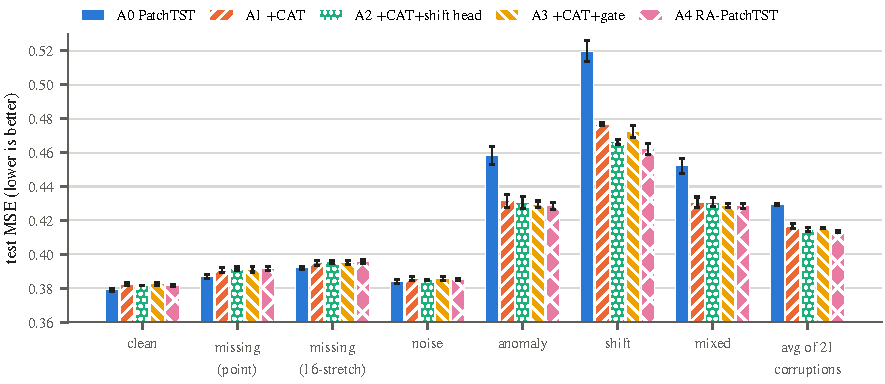
\includegraphics[width=\figwidth]{fig_mse_groups.pdf}
\caption{Test MSE by corruption family for the five variants (mean over two seeds; error bars show the standard deviation between seeds). Note that the vertical axis starts at 0.36.}
\label{fig:groups}
\end{figure*}

\subsection{Effect of RA-PatchTST (RQ2, H1)}

The full model lowers the average MSE over the 21 corrupted conditions from 0.429 to 0.413, a reduction of 3.7\% (Table~\ref{tab:delta-a0}). The reduction is 11.0\% under shift, 6.5\% under spikes and 5.2\% in the mixed setting, and the same ordering holds for MAE (Table~\ref{tab:groups-mae}). The price is a small loss elsewhere: $+0.7\%$ on clean inputs, $+1.3\%$ under point-wise missing values, $+0.9\%$ under missing stretches and $+0.2\%$ under noise. A4 beats A0 in 10 of the 21 corrupted conditions: all four spike levels, all four shift levels, the mixed setting and noise at 15\%. It is worse in the remaining eleven, all of them missing-value or low-level noise conditions where the baseline was already close to its clean error.

The improvement grows with severity (Fig.~\ref{fig:severity}). At one shifted segment A4 is 1.6\% better than A0, at ten segments 20.1\% better (0.569 against 0.712). For spikes the gain rises from 0.6\% at 1\% of points to 11.0\% at 15\%. Fig.~\ref{fig:heatmap} shows the same effect as degradation relative to each model's own clean error: A0 loses 88\% at the worst condition, A4 49\%, and averaged over the 21 conditions A0 loses 13.3\% and A4 8.3\%. For missing values the curves of the three models run nearly parallel, with A0 slightly below.

Against the success criteria of Section~\ref{sec:problem}, A4 lowers the average corrupted MSE in both seeds (0.4132 and 0.4137 against 0.4289 and 0.4298), raises clean MSE by 0.7\% (below the 2\% limit) and adds 1.2\% parameters (below 5\%). H1 is therefore supported on this dataset, with the qualification that the gain is concentrated in two corruption families.

\begin{table}[!t]
\centering
\caption{Change in Test MSE Relative to A0 (Negative Means Better)}
\label{tab:delta-a0}
\footnotesize
\colfit{%
\begin{tabular}{@{}lcccc@{}}
\toprule
Test condition & A1 & A2 & A3 & A4 \\
\midrule
\tabin{tab_delta_a0}
\bottomrule
\end{tabular}}
\end{table}

\begin{figure*}[!t]
\centering
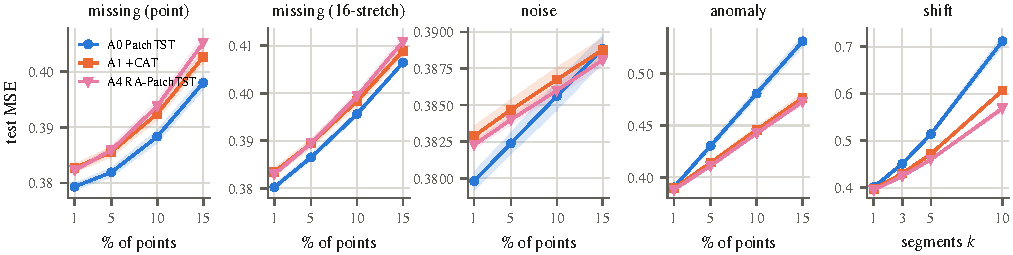
\includegraphics[width=\figwidth]{fig_severity.pdf}
\caption{Test MSE against corruption severity for A0, A1 and A4. Lines are seed means; the shaded bands span the two seeds. Note the different vertical scales.}
\label{fig:severity}
\end{figure*}

\begin{figure*}[!t]
\centering
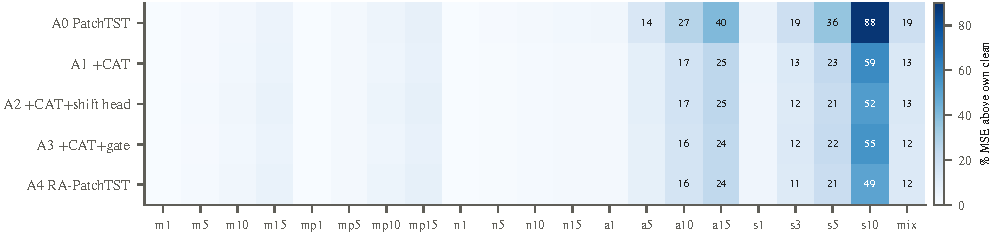
\includegraphics[width=\figwidth]{fig_heatmap.pdf}
\caption{Degradation of each variant relative to its own clean error, $100(\mathrm{MSE}_{\mathrm{cond}}/\mathrm{MSE}_{\mathrm{clean}}-1)$, for the 21 corrupted conditions (m: missing point, mp: missing 16-stretch, n: noise, a: anomaly, s: shift; numbers give the percentage level or the number of shifted segments). Cells of 10\% or more are labelled.}
\label{fig:heatmap}
\end{figure*}

\subsection{Ablation: Where Does the Gain Come From?}

Training on corrupted inputs alone (A1) already gives $-3.0\%$ of the $-3.7\%$ average reduction, that is, about four fifths of the total (Table~\ref{tab:delta-a0}, Fig.~\ref{fig:ablation}). Measured against A1 (Table~\ref{tab:delta-a1}), the shift-aware head (A2) adds $-0.5\%$ on average and $-2.2\%$ under shift, the gate (A3) adds $-0.3\%$ and $-0.9\%$, and the two together (A4) add $-0.8\%$ and $-3.0\%$. The effects of the two components add up almost exactly, which suggests that they address different parts of the problem: the head corrects the level and scale of the forecast, while the gate changes which patches the encoder relies on.

The shift-aware head is the more useful of the two architectural additions, as the analysis of RQ1 would predict: under shift the model needs the window level and scale that instance normalization removes, and the head gives them back. A2 and A4 also reach lower validation errors than A1 and A3 on both the clean and the mixed validation sets (Fig.~\ref{fig:learning}), which points to a benefit that is not limited to the test period.

\begin{table}[!t]
\centering
\caption{Change in Test MSE Relative to A1 (Corruption-Aware Training Only)}
\label{tab:delta-a1}
\footnotesize
\colfit{%
\begin{tabular}{@{}lccc@{}}
\toprule
Test condition & A2 & A3 & A4 \\
\midrule
\tabin{tab_delta_a1}
\bottomrule
\end{tabular}}
\end{table}

\begin{figure}[!t]
\centering
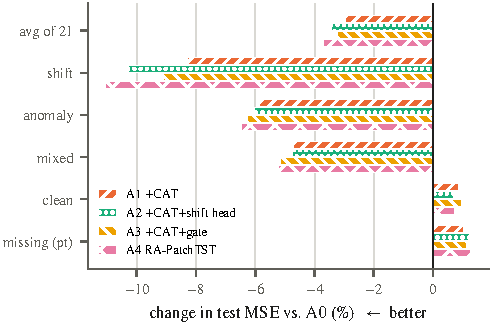
\includegraphics[width=\colfig]{fig_ablation.pdf}
\caption{Change in test MSE relative to A0 for each variant and selected condition groups. Bars to the left of zero are improvements.}
\label{fig:ablation}
\end{figure}

\subsection{Are the Differences Consistent Across Seeds?}

Table~\ref{tab:paired} compares each variant with A1 seed by seed on the average of the 21 corrupted conditions. All three variants improve on A1 in both seeds, and A4 does so by 0.0025 and 0.0039. These differences are small, of the same order as the gap between the two seeds of A1 (0.0020), and with two seeds no significance can be claimed. The comparison with A0 is on firmer ground: the difference between A0 and A4 (0.016) is about 18 times the seed spread of A0 (0.0009) and 32 times that of A4 (0.0005).

\begin{table}[!t]
\centering
\caption{Paired Per-Seed Comparison With A1 on the Average of the 21 Corrupted Conditions}
\label{tab:paired}
\footnotesize
\colfit{%
\begin{tabular}{@{}lcccl@{}}
\toprule
Variant & Seeds & Mean $\Delta$MSE & Seeds better & Per-seed $\Delta$MSE \\
\midrule
\tabin{tab_paired}
\bottomrule
\end{tabular}}
\end{table}

\subsection{Does the Gate Detect Corrupted Patches? (H2)}

Table~\ref{tab:gate} and Fig.~\ref{fig:gate-w} compare the mean gate weight on corrupted and clean patches for seven representative conditions. The gate does react to spikes: in A4 a patch containing a spike receives 0.939 on average, against 0.964 for clean patches in the same windows, and in A3 the gap is wider (0.926 against 0.963). Smaller gaps appear for shift ($-0.017$) and noise ($-0.007$). For missing values, which the zero-share feature was meant to expose, the gate hardly separates damaged from clean patches (a gap of 0.002 to 0.004).

All weights lie between 0.92 and 0.97, so the gate never comes close to switching a patch off; it behaves more like a mild global rescaling with a small extra discount on suspicious patches than like a filter. The gap is also largest for A3, where the gate is the only architectural addition, which suggests that in A4 the shift head takes over part of the work the gate would otherwise do. H2 is supported only weakly, and only for spikes. We therefore do not attribute the robustness of RA-PatchTST mainly to the gate.

\begin{table*}[!t]
\centering
\caption{Mean Gate Weight on Corrupted and Clean Patches (1.0: Fully Trusted). A Patch Counts as Corrupted if Any of Its 16 Values Was Altered}
\label{tab:gate}
\footnotesize
\begin{tabular}{@{}lccccccc@{}}
\toprule
 & & \multicolumn{3}{c}{A3 (+CAT+gate)} & \multicolumn{3}{c}{A4 (RA-PatchTST)} \\
\cmidrule(lr){3-5}\cmidrule(l){6-8}
Condition & Share corrupted & Corrupted & Clean & Gap & Corrupted & Clean & Gap \\
\midrule
\tabin{tab_gate}
\bottomrule
\end{tabular}
\end{table*}

\begin{figure*}[!t]
\centering
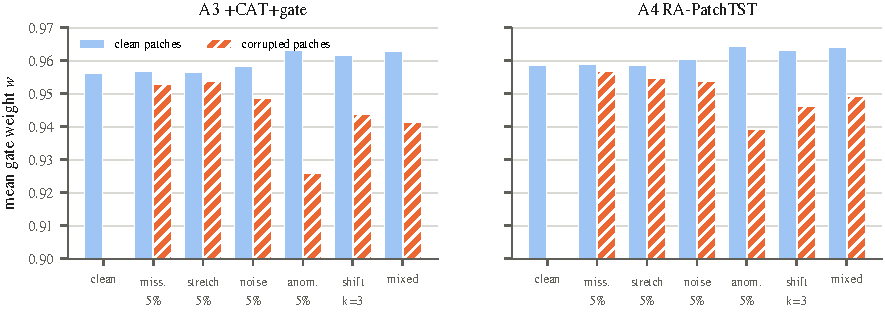
\includegraphics[width=\figwidth]{fig_gate_weights.pdf}
\caption{Mean gate weight on clean and corrupted patches for A3 and A4 (mean over two seeds). The vertical axis spans 0.90 to 0.97: every weight is close to one, and a clear gap appears only for spikes.}
\label{fig:gate-w}
\end{figure*}

\subsection{Training Dynamics}

Fig.~\ref{fig:learning} shows the validation curves. All runs used the full 20 epochs, and the selected checkpoints come from epochs 17 to 20 (Table~\ref{tab:cost}), so none of the models had clearly converged; the official schedule allows up to 100 epochs. On clean validation data A0 ends with the lowest error, as expected for the only model trained on clean data alone. On the mixed validation set the order reverses: at the selected epochs A4 reaches 0.729 to 0.734 and A0 0.761 to 0.765. In every variant the validation MSE is much higher than the test MSE (about 0.68 against 0.38 on clean data), so the two periods differ in difficulty and selection on the validation period transfers to the test period only approximately. Corruption-aware variants also end with higher training loss (0.383 to 0.388 against 0.357 to 0.358 for A0), because half of their training windows are corrupted.

\begin{figure*}[!t]
\centering
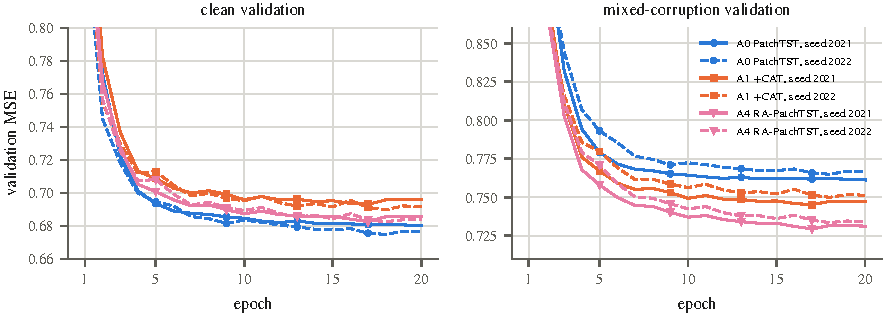
\includegraphics[width=\figwidth]{fig_learning.pdf}
\caption{Validation MSE per epoch for A0, A1 and A4 on clean (left) and mixed-corruption (right) validation windows. Solid lines: seed 2021; dashed lines: seed 2022.}
\label{fig:learning}
\end{figure*}

\subsection{Computational Cost}

Table~\ref{tab:cost} lists the cost of each variant. RA-PatchTST has 993 more parameters than PatchTST (1.2\%), of which 801 are in the gate and 192 in the head. Training time per epoch on one CPU thread rises from 37.0~s to 41.2~s ($+11\%$); 2.0~s of the increase comes from generating corruptions (A1 against A0), 2.0~s from the gate (A3 against A1) and under 1~s from the shift head (A2 against A1). Inference on the 2,785 test windows takes 4.2 to 5.5~s for all variants, and the differences between variants lie within the timing noise of a shared CPU.

\begin{table}[!t]
\centering
\caption{Model Size and Cost (Training Time on One CPU Thread; Inference Over 2,785 Test Windows)}
\label{tab:cost}
\footnotesize
\colfit{%
\begin{tabular}{@{}lrrrccc@{}}
\toprule
Variant & Params & $\Delta$ & Gate & s/epoch & Infer.\ (s) & Sel.\ epoch \\
\midrule
\tabin{tab_cost}
\bottomrule
\multicolumn{7}{@{}l@{}}{\scriptsize Sel.\ epoch: epoch of the selected checkpoint for seeds 2021/2022 (max.\ 20).}
\end{tabular}}
\end{table}

\subsection{Interactive Demonstration}

On the fixed set of 24 test windows $\times$ 7 channels in the live laboratory, with the mixed damage preset, the browser models (seed 2021) give MSE 0.433 for PatchTST and 0.426 for RA-PatchTST ($-1.5\%$), and RA-PatchTST is better on 112 of the 168 series. This is a small demonstration set and not part of the evaluation, but it agrees in direction with the test results.

\subsection{Discussion}

\subsubsection{Interpretation}
The baseline reproduces PatchTST closely and loses accuracy mainly under spikes and shift, in line with the concerns raised about window-local normalization~\cite{fan,apt,revinrole} and patch-level shift~\cite{tfps}. RA-PatchTST reduces these losses, and most of the reduction is due to the training data: a PatchTST that simply sees corrupted windows during training (A1) recovers about 80\% of the gain. The architectural additions help, mostly under shift, and the more effective of them is the simplest one, two numbers appended to the head. The gate learns to discount spikes a little but does not detect missing values.

\subsubsection{Why missing values get slightly worse}
All corruption-aware variants are 0.7 to 1.3\% worse than A0 under missing values and on clean data. Two causes are plausible. First, capacity and training signal are shared: the model spends part of both on spikes and shift, the most damaging families, at a small cost on the mild ones. Second, the zero-filling corruption is easy for the baseline to absorb (a zero is the training mean), so there is little to gain and some precision to lose. The weak response of the gate to missing values may also have a simple cause: the zero-share feature in~\eqref{eq:gatein} is one of 23 inputs, and nothing in the loss rewards the gate for using it.

\subsubsection{Practical significance}
The extra cost is small: 993 parameters, about 11\% more training time and no measurable inference overhead. For data that are mostly clean and complete, RA-PatchTST brings almost no benefit and a slight loss of accuracy. For sensors that are prone to spikes, recalibration jumps or regime changes, the reduction of up to 20\% at high shift severity is a meaningful gain. The model is a research prototype and has not been validated in operation.

\subsubsection{Limitations and threats to validity}
\label{sec:limitations}
The evidence is narrow. Only one dataset (ETTh1), one horizon (96) and one look-back (336) were tested, with two seeds and a 20-epoch budget, and no hyperparameters were tuned. No other published method was re-run, so nothing is claimed relative to SEER~\cite{seer}, TFPS~\cite{tfps}, APT~\cite{apt} or DLinear~\cite{dlinear}. The test corruptions come from the same families that were used in training (only their combination in the mixed setting is new), so the results show robustness to known corruption types, not to unseen ones. The corruptions are synthetic and may differ from real sensor faults. Test windows overlap, so naive confidence intervals would be too narrow. The differences between A2, A3, A4 and A1 are of the same order as the seed variation. Variants A5 and A6 and the gate penalty were not run, so we cannot say how the gate behaves without corruption-aware training or without the shift features. Error analysis by channel or by horizon step was not carried out.
